\documentclass[12pt]{article}
\usepackage{amsmath,amssymb,color,hyperref,graphicx,pdfsync,overpic,color,epstopdf,rotating,dashrule,float,bm}
\begin{document}
\bibliographystyle{plain}

\title{\textbf{\Large SPH: A Smoothed Particle Hydrodynamics code} \\ User Guide}
\author{Anthony DeGennaro, Kevin Nowland, Scott Dawson \\ and Im\`ene Goumiri}
\date{18 January 2013}
%\begin{figure}
%\begin{center}
%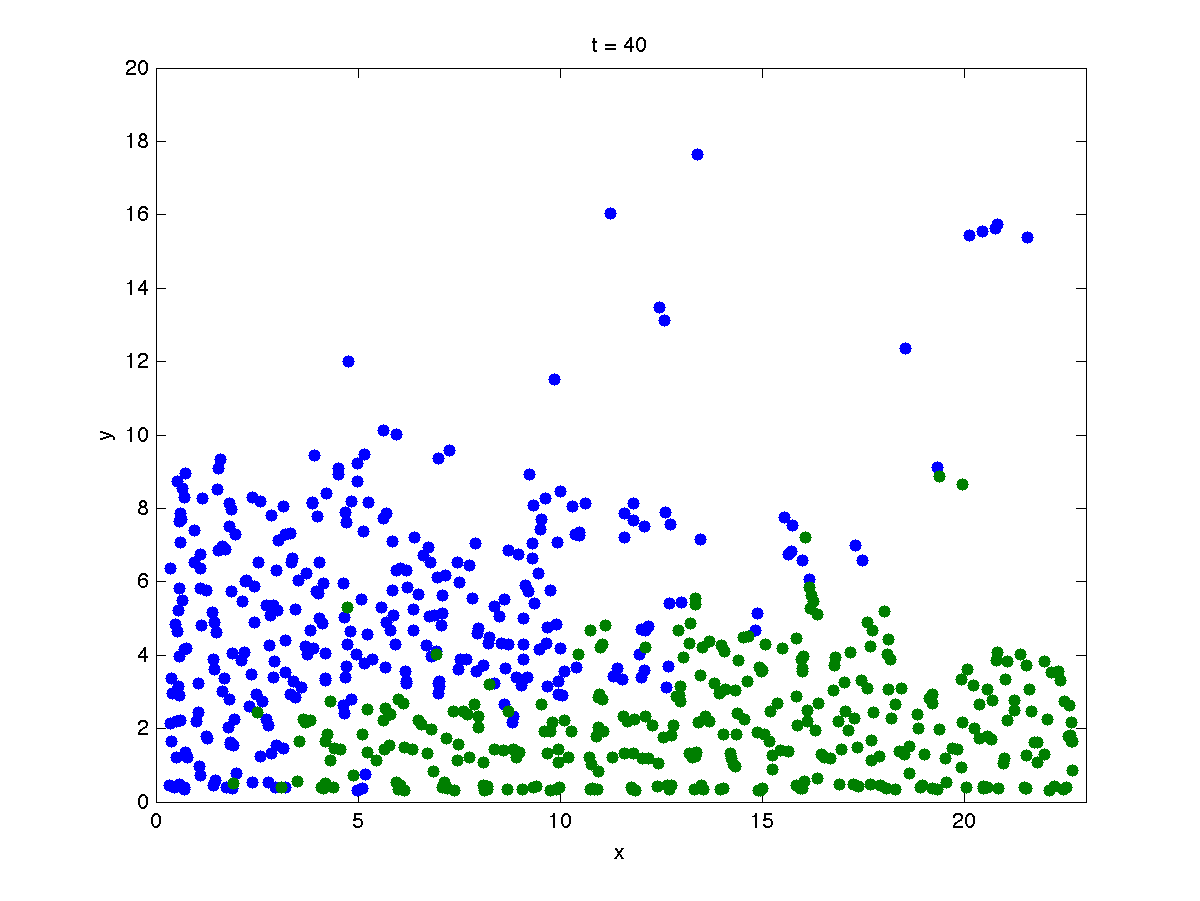
\includegraphics[width= 0.8\textwidth]{SpheresDiffdensities_401.pdf}
%
%\end{center}
%\end{figure}
\maketitle


\section{Introduction}

This code uses smoothed particle hydrodynamics (SPH) to simulate the flow of (approximately) incompressible fluid. Unlike many grid-based fluids solvers, SPH operates by tracking individual ``particles" or clumps of fluid. This makes SPH useful for a variety of flows for which fixed grid based methods are difficult to implement, such as flows involving highly deforming free surfaces.

\section{Compiling}
After downloading the source code, the main executable \texttt{sph} can be compiled simply by running make. The code requires that the user have Boost libraries installed (available at http://sourceforge.net/projects/boost/files/boost/1.52.0/). The \texttt{Makefile} also generates the executable file \texttt{tests}, which runs google tests for various important functions in the code. This requires that google tests be installed (available at http://code.google.com/p/googletest/). 

Important in compiling is linking to the \texttt{boost} library and 
\texttt{gtest}. After installing these libraries, the user should set two
environment variables, one called \texttt{BOOST} and one called 
\texttt{GTEST}. For example, using \texttt{bash} on Ubuntu 12.04, the
following commands sufficed:

\texttt{\$  GTEST=/usr/src/gtest/include/}

\texttt{\$  export GTEST}
  
\texttt{\$  BOOST=/usr/local/boost\_1\_52\_0}

\texttt{\$ export BOOST}

\noindent
To enable compiler optimization, set \texttt{NDEBUG=1} before \texttt{make}.


\section{Running the Code}

The input syntax for running \texttt{sph} is as follows:

\begin{center} \texttt{sph <initFile> <boundaryFile(OPTIONAL)> <tfinal> <timestep> <integratorType> <kernelType>} \end{center}
The data files \texttt{initFile} and \texttt{boundaryFile} provide information about the fluid and boundary particles, and have the syntax:
%
\begin{description}
	\item[``INPUT.DAT"]
		\begin{verbatim}

[Total Number of Particles]

[Number] x y u v [Mass] [Density] [Pressure] [Energy]
                     . . . . . . .
                     . . . . . . .
		\end{verbatim}
\end{description}
 
Here, the particle numbering should begin at zero, and {x, y, u, v} specify the initial position and velocity components in a 2-D plane. The user may obviously generate the initial conditions in these input files by means of whatever pre-processing routines they desire (for example, a simple MatLab script to generate specific initial/boundary conditions often is a quick and nice solution). Since the code is currently restricted to incompressible fluids, the energy property is not presently used. For boundary particles, none of the mass, density, pressure and energy values are used, though this could change if the method of interaction between the particles and the boundary is handled differently in a different physics class.

Three types of integrator are provided, which are selected in the command line by:
\begin{itemize}
\item \texttt{euler}, a standard forward stepping Euler routine
\item \texttt{eulermod}, which uses the Euler method, but updating particle positions using the already
updated velocity values.
\item \texttt{pc}, a second order predictor corrector algorithm, based on that outlined in \cite{Price04}.
\end{itemize}

When chosing the appropriate timestep, the user must keep in mind that simulations will not necessarily `break' if the timestep is too large to be accurate, so it is important to verify that the timestep chosen is sufficiently small. This can be attained either by ad-hoc convergence testing, or with reference to the Courant condition, which states that the maximum timestep to retain accuracy is 
$$ dt_c = C_{cour} \min\left(\frac{h}{v}\right),$$
where $C_{cour}$ is a constant that is often taken to be  $0.4$, and $h$ and $v$ are typical relative particle spacings and velocities, respectively. In reality, effects such as interactions with boundaries can interfere with the validity of this condition, so we reccomend that the user verifies the accuracy of their chosen timestep. As a rule of thumb, a timestep of $0.001$ when using the \texttt{euler} method is more than sufficient for all of the testcases provided (which can be increased for the \texttt{pc} method). The user also has a choice between the use of \texttt{spline} and \texttt{gaussian} kernels.

As well as the parameters inputted in the command line, there are additional properties that can be edited within \texttt{sph.cc} itself, which concern the properties of the fluid - namely the coefficients in the equation of state and viscosity calculation. These have been set to typical values for water. Also inputted is the desired smoothing length, which should be about twice the typical particle spacing. These properties are defined when creating an instance of the physics class. For further details of the code structure, refer to the Doxygen documentation and final report.

Output is handled in a manner which closely resembles the input protocol. Specifically, at regular intervals (which can be specified in the driver program), the SPH code writes the full state information of each fluid particle to a pre-specified output file. The output syntax is as follows:

\begin{description}
	\item[``OUTPUT.DAT"]
		\begin{verbatim}

[Timestep 1]

[Number] x y u v [Mass] [Density] [Pressure] [Energy]
                     . . . . . . .
                     . . . . . . .

[Timestep 2]

[Number] x y u v [Mass] [Density] [Pressure] [Energy]
                     . . . . . . .
                     . . . . . . .
		\end{verbatim}
\end{description}
	
Example input and output files are included in the \texttt{TESTCASES} folder, along with a readme document explaining typical usage. Also included is a sample Matlab script that can be used to visualize the particle locations (obtained from the output file) evolving with time.
\\
\\
Some additional Tips:
\begin{itemize}
\item As has been reported in the literature, Spline kernels typically give better results that Gaussian kernels.
\item Initial particle spacing should be approximately 0.5 smoothing lengths (note that this is for our implementation - there are numerous definitions of smoothing length in the literature).
\item If the user changes the definition of \texttt{Fluid::findNeighbors} the test may fail, as this test was written with the mesh method in mind. In particular, implementing the naive comparison of each particle to every other particle will cause this test to fail.
\end{itemize}

\bibliography{refs}
\end{document}
